\scanpage{118}
\mspage{117}


$\unsure{\otimes|\Omega}$-\uline{categories}.

1) Definition. \deleted{Additiv} Additive category, with bifunctor
\[
(X,Y)\handwritten{\mapsto}X\otimes Y
\]
\deleted{and} an \deleted{object} isomorphism of bifunctors
\[
\handwritten{\phi}(X,Y,Z): (X\otimes Y)\otimes Z\handwritten{\xrightarrow{\sim}}X\otimes(Y\otimes Z)
\]
and a commutativity isomorphism
\[
\handwritten{\unsure{\mu|\psi}}(X,Y): X\otimes Y\handwritten{\xrightarrow{\sim}}Y\otimes X
\]
satisfying axioms

a) Pentagon axiom for $\handwritten{\phi}$ \deleted{(does not depend on the additive structure),}

b) $\handwritten{\mu}(X,Y)\handwritten{\mu}(Y,X)=\mathrm{id}_{\unsure{\rlap{Y}X|X}\otimes X}$ \handwritten{;}

c) compatibility between $\handwritten{\phi}$ and $\handwritten{\mu}$ \handwritten{; hexagon axiom}

d) existence of an element $1_C=\underline{1}$ , with functorial isomorphisms
\[
u(X):\deleted{\unsure{x}}\quad\underline{1}\otimes X\handwritten{\simeq}X
\qquad\text{whence}\quad
\inserted{v(X)=}\handwritten{\mu}(X,1)u(X): X\otimes1\handwritten{\simeq}X\ ,
\]
\figure{\handwritten{
\begin{tikzpicture}[x=1cm,y=1cm]
\draw (-.75,.05) .. controls (-.9,.7) and (.3,.3) .. (.5,.6);
\draw (-.6,.05) .. controls (-.4,-.45) and (.75,-.4) .. (.85,0) .. controls (.95,.6) and (1.5,.7) .. (1.85,.3);
\draw[line width=.15pt] (1.12,.57)--(1.48,.28);
\draw[line width=.15pt] (.03,-.49) .. controls (.29,-.63) and (.56,-.52) .. (.69,-.43);
\end{tikzpicture}}}
% The preceding figure records the transposition/enclosure strokes on the two factors; the typed order is retained in the display.
(thus, by b we shall also have $u(X)=v(X)\handwritten{\mu}(1,X)$)

with the condition that for $X=\underline{1}$, one finds the same isomorphism
\[
\makebox[0pt][r]{\begin{tikzpicture}[x=1em,y=1em]\fill (0,0) circle (.045);\end{tikzpicture}\hspace{3em}}
u(\underline{1})=v(\underline{1}) :\qquad \underline{1}\otimes\underline{1}\handwritten{\simeq}\underline{1}
\]
which is also expressed by the condition that $\handwritten{\mu}(\underline{1},\underline{1})=\mathrm{id}_{\underline{1}}$ \handwritten{;}

\margin{\handwritten{\figure{
\begin{tikzpicture}[x=1cm,y=1cm]
\node[align=left] at (0,0) {moreover we want};
\draw (-1.23,-.23) .. controls (-1.8,.03) and (-1.62,.62) .. (-1.16,.65) -- (1.22,.81) .. controls (1.61,.83) and (1.77,.08) .. (1.53,-.03) -- (-.82,-.25) .. controls (-1.3,-.35) and (-1.5,-.76) .. (-1.25,-1.09);
\end{tikzpicture}}}}
\inserted{\handwritten{Compatibility of $(\underline{1},u,v)$ with $\phi$, when $X,Y$ \unsure{,-|or} $Z$ \unsure{is} \unsure{equal|equal} to $1$, with $\mu$ when $X$ \unsure{,-|or} $Y$ is $=1$.}}

e) the functor $\otimes$ is biadditive.

\margin{\handwritten{\figure{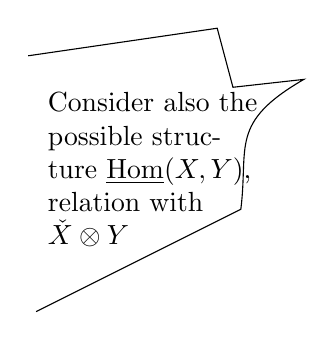
\begin{tikzpicture}[x=1cm,y=1cm]
\node[align=left,text width=2.7cm] at (0,0) {Consider also the possible structure $\underline{\mathrm{Hom}}(X,Y)$, relation with $\check{X}\otimes Y$};
\draw (-1.6,1.45) -- (.8,1.8) -- (1,1.05) -- (1.9,1.15) .. controls (.95,.6) and (1.2,.3) .. (1.1,-.5) -- (-1.5,-1.8);
\end{tikzpicture}}}}

NB a) \deleted{and d) are}\inserted{is} independent\deleted{s} of the datum of $\handwritten{\mu}$ , b) is independent of the datum of $\handwritten{\phi}$ , a)b)c)d) are independent of th\unsure{\rlap{u}e|e} fact that $C$ is additiv\deleted{\unsure{t}}e.

Let $\underline{1}',u',\inserted{v'\handwritten{\begin{tikzpicture}[x=.4cm,y=.4cm,baseline=-.2ex]\draw (0,-.2) .. controls (-.28,.4) and (.1,.65) .. (.53,1.01);\end{tikzpicture}}}$ be as $\underline{1},u,v$ , we shall \deleted{canonically define an}\inserted{\handwritten{see that there exists a unique}} isomorphism $w:\underline{1}\handwritten{\simeq}\underline{1}'$ , compati\unsure{\rlap{v}b|b}le in an obvious sense with $u,v$ and $u',v'$.

We choose the composite
\diagram{\begin{tikzcd}[ampersand replacement=\&]
\underline{1} \arrow[r,"{\handwritten{v'(\underline{1})}}"] \&
\underline{1}\otimes\underline{1}' \arrow[r,"{\handwritten{\unsure{\rlap{\(\underline{1}\otimes u'\)}u(\underline{1}')|u(\underline{1}')}}}"] \&
\underline{1}'\deleted{\otimes\unsure{\underline{1}}} \arrow[r,phantom,"{\deleted{\longrightarrow}}" description,"{\deleted{\handwritten{\unsure{u}}}}"] \& \deleted{\unsure{\underline{1}'}}
\end{tikzcd}}
. To check the stated compatibilities (does not depend on the datum of $\handwritten{\phi}$, \inserted{nor $\handwritten{\mu}$,\handwritten{\begin{tikzpicture}[x=.4cm,y=.4cm,baseline=-.2ex]\draw (0,-.2) .. controls (-.18,.36) and (.2,.46) .. (.42,.48) .. controls (.93,.5) and (1.34,.62) .. (1.27,.79);\end{tikzpicture}}} but on $u,v$ satisfying the compatibility $\underline{u}(\underline{1})=v(\underline{1})$\deleted{\unsure{\mbox{
\begin{tikzpicture}[x=.5em,y=.5em,baseline=-.2ex]
\draw (.17,.57) ellipse (.16 and .21);
\draw (.08,-.25) .. controls (.28,.05) and (.17,.76) .. (.13,1.02);
\draw (.13,1.02) .. controls (.18,.91) and (.3,.91) .. (.38,1.04);
\draw (.23,.73)--(.43,.79);
\draw (.81,.61)--(.48,.24)--(.79,.24) .. controls (1,.08) and (.76,-.08) .. (.68,-.05);
\end{tikzpicture}}|,}} and $u',v'$ ditto). That is why there \inserted{is\handwritten{\begin{tikzpicture}[x=.4cm,y=.4cm,baseline=-.2ex]\draw (0,-.2) .. controls (.05,.21) and (.31,.65) .. (.53,.94);\end{tikzpicture}}} no need to posit $\underline{1},u,v$ as a datum, but as an existence axiom.
